\section{Materials and Methods}\label{sec:methods}

\subsection{Dataset, Target, and Feature Representation}

The empirical dataset contains 15,057 clean, chronologically ordered five-minute bars for B3 Mini-Index futures (WIN), drawn from BovDB resources \cite{cardoso2022bovdb,souza2024dataset}. The binary target is the next-bar directional movement, with $y_k=1$ for an uptrend and $y_k=0$ otherwise. The source pipeline derives 66 price-, moving-average-, volatility-, volume-, and trade-frequency descriptors. In keeping with the precursor, Information Gain selects seven descriptors: two EMA differences, their normalized counterparts, normalized SMA$_9$, EMA$_{9-3}$, and normalized EMA$_7$. This preserves the predecessor's compact feature representation while changing the validation and optimizer design.

\subsection{Temporal Protocol and Shared Search Controls}

All runs follow the same chronological 60/20/20 partition: the first 9,034 bars form the training block, the following 3,011 bars form the validation block, and the final 3,012 bars form the locked test block. No shuffling is applied. The test block is never used to rank candidates or select a fitness function.

Four classifier backbones are assessed: MLP, Random Forest, SVM, and 1D-CNN. Their hyperparameters cover architecture size, regularization, learning rate, dropout, batch size, tree settings, and kernel settings. Each backbone is searched by RS, GA, PSO, DE, and GWO. To make their comparisons interpretable, every optimizer receives the same candidate-evaluation allowance:
\begin{equation}\label{eq:budget}
N_{\mathrm{eval}}=1{,}000 \quad \text{evaluations per optimizer and seed}.
\end{equation}

The optimizers retain their standard search roles: RS samples feasible configurations; GA uses tournament selection, crossover, and mutation; PSO uses cognitive and social attraction; DE uses differential perturbation and crossover; and GWO updates a population through its $\alpha$, $\beta$, and $\delta$ leaders. The purpose is not to tune their internal operators asymmetrically, but to compare their model-selection behaviour under the same evaluation opportunity.

\subsection{Dual-Fitness Design}

Figure~\ref{fig:workflow} depicts the controlled comparison. Protocol A ranks candidates on the validation block by a compound imbalance-aware fitness,
\begin{equation}\label{eq:mcc_fitness}
f_{\mathrm{MCC/F1}}(\boldsymbol{\theta})=0.60\,\mathrm{MCC}_{\mathrm{val}}(\boldsymbol{\theta})+0.40\,F_{1,\mathrm{val}}(\boldsymbol{\theta}),
\end{equation}
whereas Protocol B ranks candidates by a weighted training/validation accuracy,
\begin{equation}\label{eq:accuracy_fitness}
f_{\mathrm{Acc}}(\boldsymbol{\theta})=0.40\,\mathrm{Accuracy}_{\mathrm{train}}(\boldsymbol{\theta})+0.60\,\mathrm{Accuracy}_{\mathrm{val}}(\boldsymbol{\theta}).
\end{equation}

The protocols differ only in this validation objective. Data, features, model families, optimizer families, budget, and test block are shared. After selection, both protocols report test MCC, test accuracy, and test $F_1$.

\begin{figure}[htbp]
\centering
\resizebox{0.96\linewidth}{!}{%
\begin{tikzpicture}[
  node distance=0.72cm and 0.62cm,
  every node/.style={
    draw=black!80,
    rounded corners=2.5pt,
    align=center,
    minimum height=0.88cm,
    text width=2.75cm,
    font=\footnotesize
  },
  process/.style={fill=black!5},
  protocol/.style={fill=black!12, text width=3.15cm},
  outcome/.style={fill=black!18, text width=4.10cm},
  arrow/.style={-{Stealth[length=2.0mm]}, thick}
]
  \node[process] (data) {\textbf{Input data}\\WIN five-minute futures\\$N=15{,}057$ bars};
  \node[process, right=of data] (indicators) {\textbf{Technical indicators}\\66 price, moving-average, volatility, volume, and trading descriptors};
  \node[process, right=of indicators] (selection) {\textbf{Feature selection}\\Information Gain\\seven retained features};

  \node[process, below=1.05cm of indicators] (split) {\textbf{Temporal data partition}\\chronological 60/20/20\\train, validation, locked test};
  \node[process, below=of split] (search) {\textbf{Equal-budget optimizer search}\\RS, GA, PSO, DE, and GWO\\$N_{\mathrm{eval}}=1{,}000$ per seed};

  \node[protocol, below left=0.92cm and 0.25cm of search] (mcc) {\textbf{Protocol A: MCC/$F_1$ fitness}\\$0.60\,\mathrm{MCC}_{\mathrm{val}}+0.40\,F_{1,\mathrm{val}}$};
  \node[protocol, below right=0.92cm and 0.25cm of search] (accuracy) {\textbf{Protocol B: accuracy fitness}\\$0.40\,\mathrm{Acc}_{\mathrm{train}}+0.60\,\mathrm{Acc}_{\mathrm{val}}$};
  \coordinate (protocolmid) at ($(mcc.south)!0.5!(accuracy.south)$);
  \node[outcome, below=1.00cm of protocolmid] (test) {\textbf{Model fitting and locked evaluation}\\RF, SVM, MLP, and 1D-CNN; common seeds 1--3\\held-out accuracy, MCC, $F_1$, and intraday economic evaluation};

  \draw[arrow] (data) -- (indicators);
  \draw[arrow] (indicators) -- (selection);
  \draw[arrow] (selection.south) |- (split.east);
  \draw[arrow] (split) -- (search);
  \draw[arrow] (search) -- (mcc);
  \draw[arrow] (search) -- (accuracy);
  \draw[arrow] (mcc.south) |- (test.west);
  \draw[arrow] (accuracy.south) |- (test.east);
\end{tikzpicture}%
}
\caption{Overview of the proposed methodology. The pipeline retains the precursor's sequence of intraday data preparation, indicator construction, feature selection, model fitting, and final evaluation; the new benchmark inserts a chronological partition, equal-budget optimizer comparison, and two explicitly separated validation objectives.}
\label{fig:workflow}
\end{figure}

\begin{figure}[htbp]
\centering
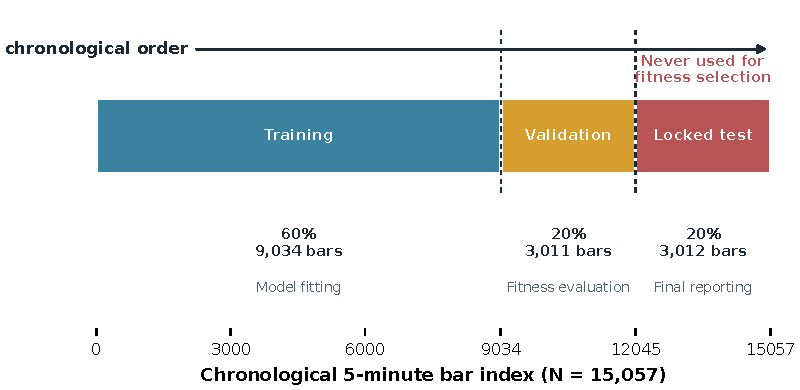
\includegraphics[width=0.86\linewidth]{figures/dual_fitness_temporal_split.pdf}
\caption{Chronological 60/20/20 partition. The final test block is unavailable during feature fitting, candidate ranking, and hyperparameter selection.}
\label{fig:temporal_split}
\end{figure}

\subsection{Evidence Scope, Statistical Analysis, and Economic Evaluation}

Three seeds (1--3) are available for every model--optimizer combination in both protocols. Therefore, the direct protocol contrast uses 20 cell means per protocol, each averaged over the same three seeds, and is presented descriptively. It is not a 20-seed confirmatory test of one fitness against another.

A complementary model-level analysis is performed within each holdout protocol. The five optimizer--seed combinations form 15 matched blocks for the four model backbones. Friedman tests assess global rank differences, followed by paired Wilcoxon tests with Holm adjustment for post-hoc MLP contrasts. This analysis answers whether models separate within a fixed protocol; it does not infer a global fitness advantage.

Finally, the locked predictions are evaluated through an intraday long/short trading simulation. The analysis reports total profit, profit factor, annualized Sharpe ratio, and maximum drawdown. Economic results are interpreted jointly with predictive metrics because a trading strategy can have different return and drawdown characteristics despite similar classification accuracy.
